\documentclass[10pt,letterpaper]{article}

\usepackage{cogsci}
\usepackage{pslatex}
\usepackage{apacite}
\usepackage{graphicx}

\title{Excessively costly degree adverbs are stronger than quite costly ones}
 
\author{
% {\large \bf Erin Bennett (erindb@stanford.edu)} \\
%   Department of Psychology, 450 Serra Mall \\
%   Stanford, CA 94305 USA
%   \AND {\large \bf Justine T. Kao (justinek@stanford.edu)} \\
%   Department of Psychology, 450 Serra Mall \\
%   Stanford, CA 94305 USA
%   \AND {\large \bf Noah D. Goodman (ngoodman@stanford.edu)} \\
%   Department of Psychology, 450 Serra Mall \\
%   Stanford, CA 94305 USA
  }

\begin{document}

\maketitle

\begin{abstract}
Different words have different production costs assosiated with them, due to their length or infrequency. We find evidence that these costs at least partially predict the strength of the meanings of different degree adverbs.
% Can word frequency predict the meanings of degree adverbs? We provide some evidence that the meaning of a degree adjective might be at least in part determined by the cost uttering that degree adverb, where more surprising, lengthly degree adverbs are more costly.

\textbf{Keywords:} 
degree adverbs; word frequency.
\end{abstract}

\section{Introduction}

Degree adverbs are adverbs that modify scalar adjectives by increasing or decreasing the extent to which that adjective applies. For example, ``very'' and ``extremely'' are degree adverbs that intensify the adjectives they modify, and ``moderately'' and ``sorta'' are degree adverbs that deintensify the adjectives they modify.

How do we know how much a degree adverb will modify an adjective's meaning? In this paper, we hypothesize that communicative pressures might determine the meanings of these degree adverbs: those that are easier to retrieve from memory and to say will have correspondingly weaker meanings, and those that are more costly to utter will have stronger meanings. This hypothesis predicts that longer degree adverbs will have stronger meanings, but also that the more commonly used a particular degree adverb is (and therefore the more accessible it is) the weaker its meaning will become.

%We hypothesize that the strength of a degree adverb is at least in part determined by the cost of uttering that adverb: degree adverbs that are more surprising or longer will be slightly more difficult to say or process, would therefore have higher communicative costs, and would consequently have stronger meanings.

\citeA{lewis} found that longer words tend to have more complex meanings associated with them, and learners tend to use this information in interpreting novel words. They hypothesized that lexicalized in-the-moment communicative pressures might be responsible for this complexity bias.

%They offer three hypotheses as to why this might be the case: \emph{innate bias}, \emph{efficient naming}, and \emph{communicative pressure}. Only the last of these would predict that 

%this might be a kind of lexicalized pragmatic inference.

%The mechanism behind this might be pragmatic inference: if the speaker went through the trouble of saying such a long word, they must be trying to communicate an especially unusual meaning.

% In several correlational studies, we check whether the frequency of degree adverbs in a corpus and/or their length in syllables can predict the prices of objects labeled as ``[adverb] expensive''. In Experiment 1, we first look at intensifying degree adverbs, for which stronger meanings would imply higher prices (``extremely expensive'' is probably more expensive than ``expensive''). In Experiment 2, we look at deintensifying degree adverbs, for which stronger meanings would imply lower prices (``kinda expensive'' is probably less expensive than ``expensive''). In Experiment 3, we study both kinds of degree adverbs together and find similar (although less strong) results.
% 
% %this might be a lexicalized pragmatic inference
% 
% % Degree adverbs are adverbs that modify the degree to which a particular adjective applies, for example ``very'', ``extremely'', ``moderately'', or ``kinda''. We will call degree adverbs that increase the extent to which an adjective applies (e.g. ``very'') \emph{intensifying} degree adverbs, and those that lessen the extent to which an adjective applies \emph{deintensifying} degree adverbs.
% % 
% % We hypothesize that the meaning of these adverbs is derived, at least in part, from the cost to the speaker of choosing a particular adverb over another. This cost is influenced by the frequency with which that adverb is used (frequent adverbs are less costly and infrequent adverbs are more costly), and by the length of the word (longer words or phrases are more costly than shorter ones). Therefore, by our hypothesis, degree adverbs that are short and common will modify adjective meanings only a small amount, but degree adverbs that are very long and uncommon will modify adjective meanings much more.
% % 
% % We test this hypothesis by eliciting interpretations of different degree adverbs when combined with the adjective ``expensive'' and comparing these interpretations to the adverbs' syllable length and corpus frequencies.
% 
\section{Experiment 1: intensifiers}

  In Experiment 1, we tested whether intensifying degree adverbs have stronger meanings (higher prices when paired with ``expensive'') when they have higher communicative cost.
  
  We consider surprisal and length in syllables as possible sources of communicative cost. We calculate the surprisal of a word ($-log(P(word))$) by approximating the probability of a word as the proportion of occurances in the Google Web 1T 5-grams database \cite{web1t5gram}.
  
  \subsection{Method}
    \subsubsection{Participants}
      We recruited 40 participants on Amazon's Mechanical Turk.
    \subsubsection{Procedure and Materials}
      We showed each participant every combination of 3 items (\emph{laptop}, \emph{watch}, and \emph{coffee maker}) and 16 intensifying degree adverbs (Table~\ref{intensifiers-table}) with the adjective ``expensive''. Each participant also saw each item described only by the adjective ``expensive'' and no degree adverb. For each of these combinations of item and degree adverb, we elicited a free response price that the participant thought the item being described might have (Figure~\ref{screenshot-figure}).
      
       As is the case for most words, the surprisals and syllable lengths of these degree adverbs were highly correlated (0.6809494).
      
      \begin{table}[!ht]
      \begin{center} 
      \caption{Intensifying degree adverbs from Experiment 1.} 
      \label{intensifiers-table} 
      \vskip 0.12in
      \begin{tabular}{lrr} 
      \hline
      Intensifier    &  Frequency & Syllable length \\
      \hline
      very & 292897993 & 2 \\ 
      really & 148918637 & 2 \\ 
      quite & 55269390 & 1 \\ 
      extremely & 21862963 & 3 \\ 
      super & 16902202 & 2 \\ 
      crazy & 13048828 & 2 \\ 
      terribly & 1906059 & 3 \\ 
      wildly & 1414395 & 3 \\ 
      vastly & 1311113 & 2 \\ 
      hugely & 1074430 & 2 \\ 
      enormously & 1011751 & 4 \\ 
      exceedingly & 977435 & 4 \\ 
      excessively & 877280 & 4 \\ 
      horribly & 819111 & 3 \\ 
      insanely & 359644 & 3 \\ 
      uncommonly & 135747 & 4 \\
      \hline
      \end{tabular} 
      \end{center} 
      \end{table}
    
      \begin{figure}[ht]
      \begin{center}
      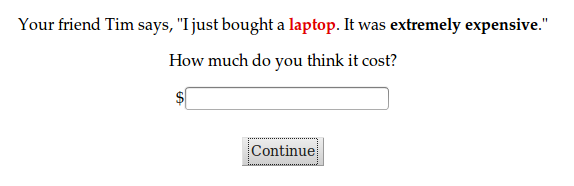
\includegraphics[width=0.45\textwidth]{screenshot.png}
      \end{center}
      \caption{Free response elicititation from Experiment 1.}
      \label{screenshot-figure}
      \end{figure}
      
    \subsubsection{Experiment 1B: prior elicitation}
      We ran an additional experiment on a separate set of participants who gave us prices for different items. These prices were elicited with free response (Figure~\ref{screenshot2}) and from this we computed means and standard deviations of people's distributions over prices for the items in our experiments.
      
      \begin{figure}[ht]
      \begin{center}
      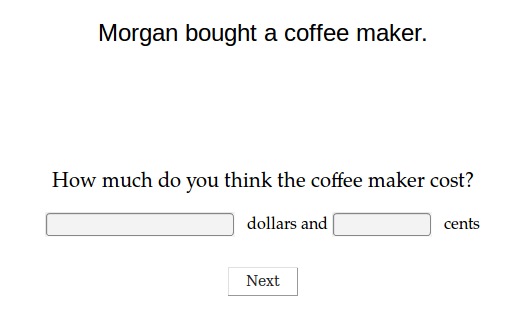
\includegraphics[width=0.45\textwidth]{screenshot2.png}
      \end{center}
      \caption{Free response price prior elicititation from Experiment 1B.}
      \label{screenshot2}
      \end{figure}
      
  \subsubsection{Results}
  
  In a mixed effects linear model of the raw data with fixed effects of surprisal and syllable length and random effects of item and participant, we found no significant effect of either surprisal or syllable length on participants' responses (Figure~\ref{raw-figure}, surprisal: estimate=602, p=0.5551906; syllable length: estimate=-208, p=0.9203443).
  
  However, when we augment our data with results of the separate prior elicitation experiment (Experiment 1B), we do see significant positive effects of both surprisal and syllable length (Figure~\ref{scaled-figure}, surprisal: estimate=0.1884, p=4.2e-07; syllable length: estimate=0.7187, p=0.00023).\footnote{We also see a significant negative interaction between the two measures, apparently because of the item ``uncommonly'', which has many syllables and shows up rarely in the Google Web 1T 5-gram corpus, but is nonetheless given a relatively low price estimate by participants.}
  
  \begin{figure}[ht]
  \begin{center}
  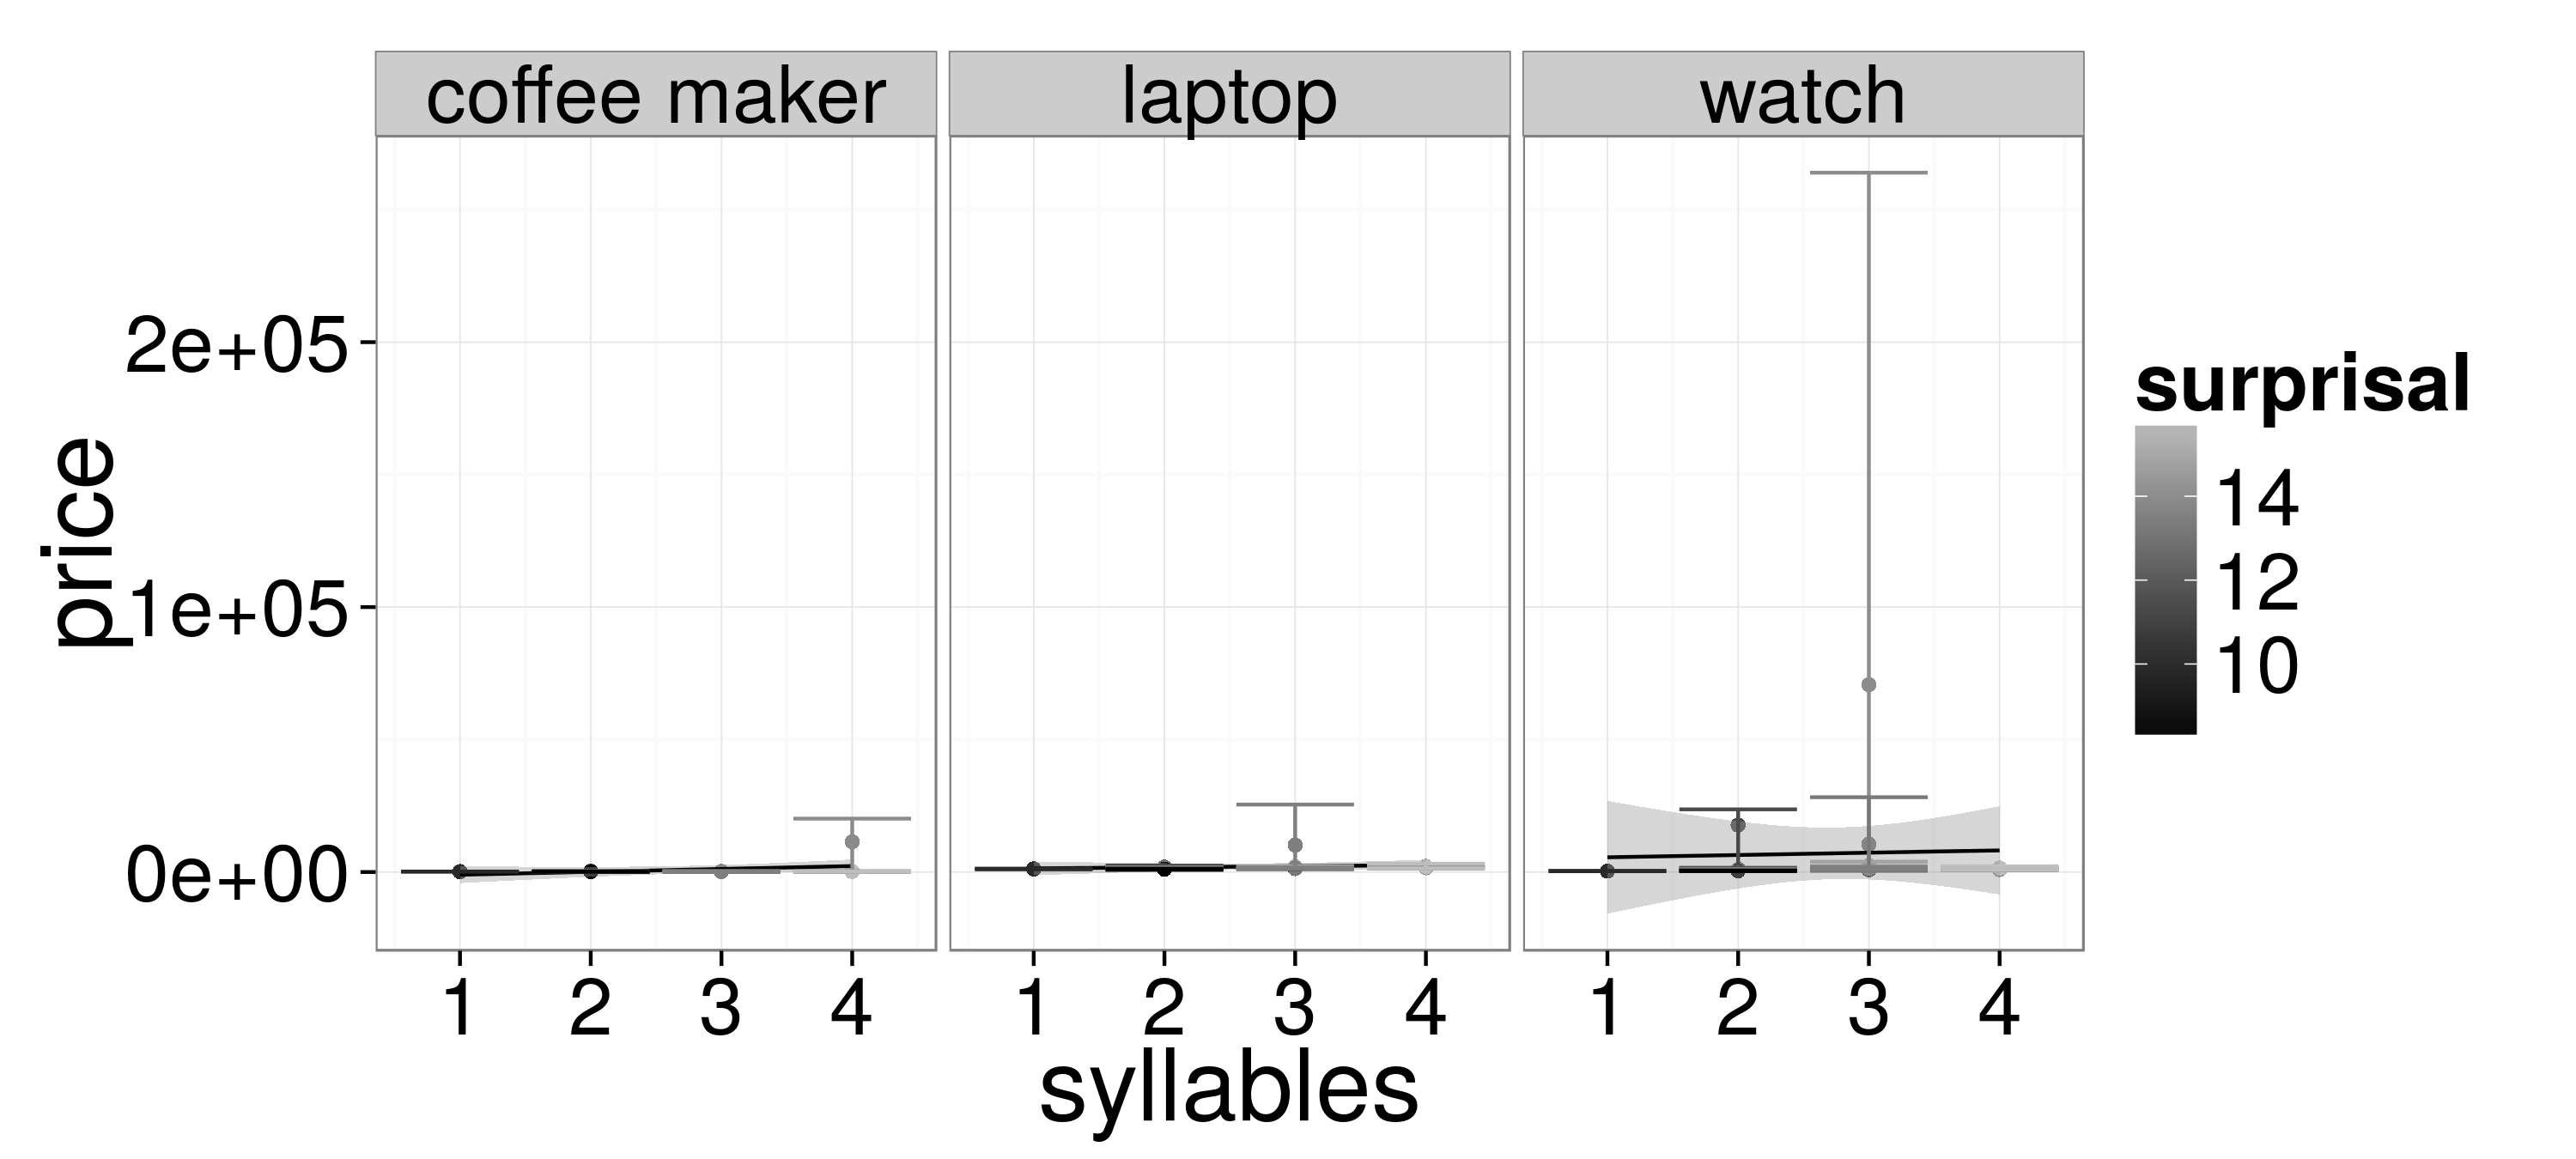
\includegraphics[width=0.45\textwidth]{exp1-raw-syllables.png}
  \end{center}
  \caption{Syllable length versus response in raw data from Experiment 1. Between participants variation in scale, as well as between item differences, make these data difficult to interpret.} 
  \label{raw-figure}
  \end{figure}
  
  \begin{figure}[ht]
  \begin{center}
  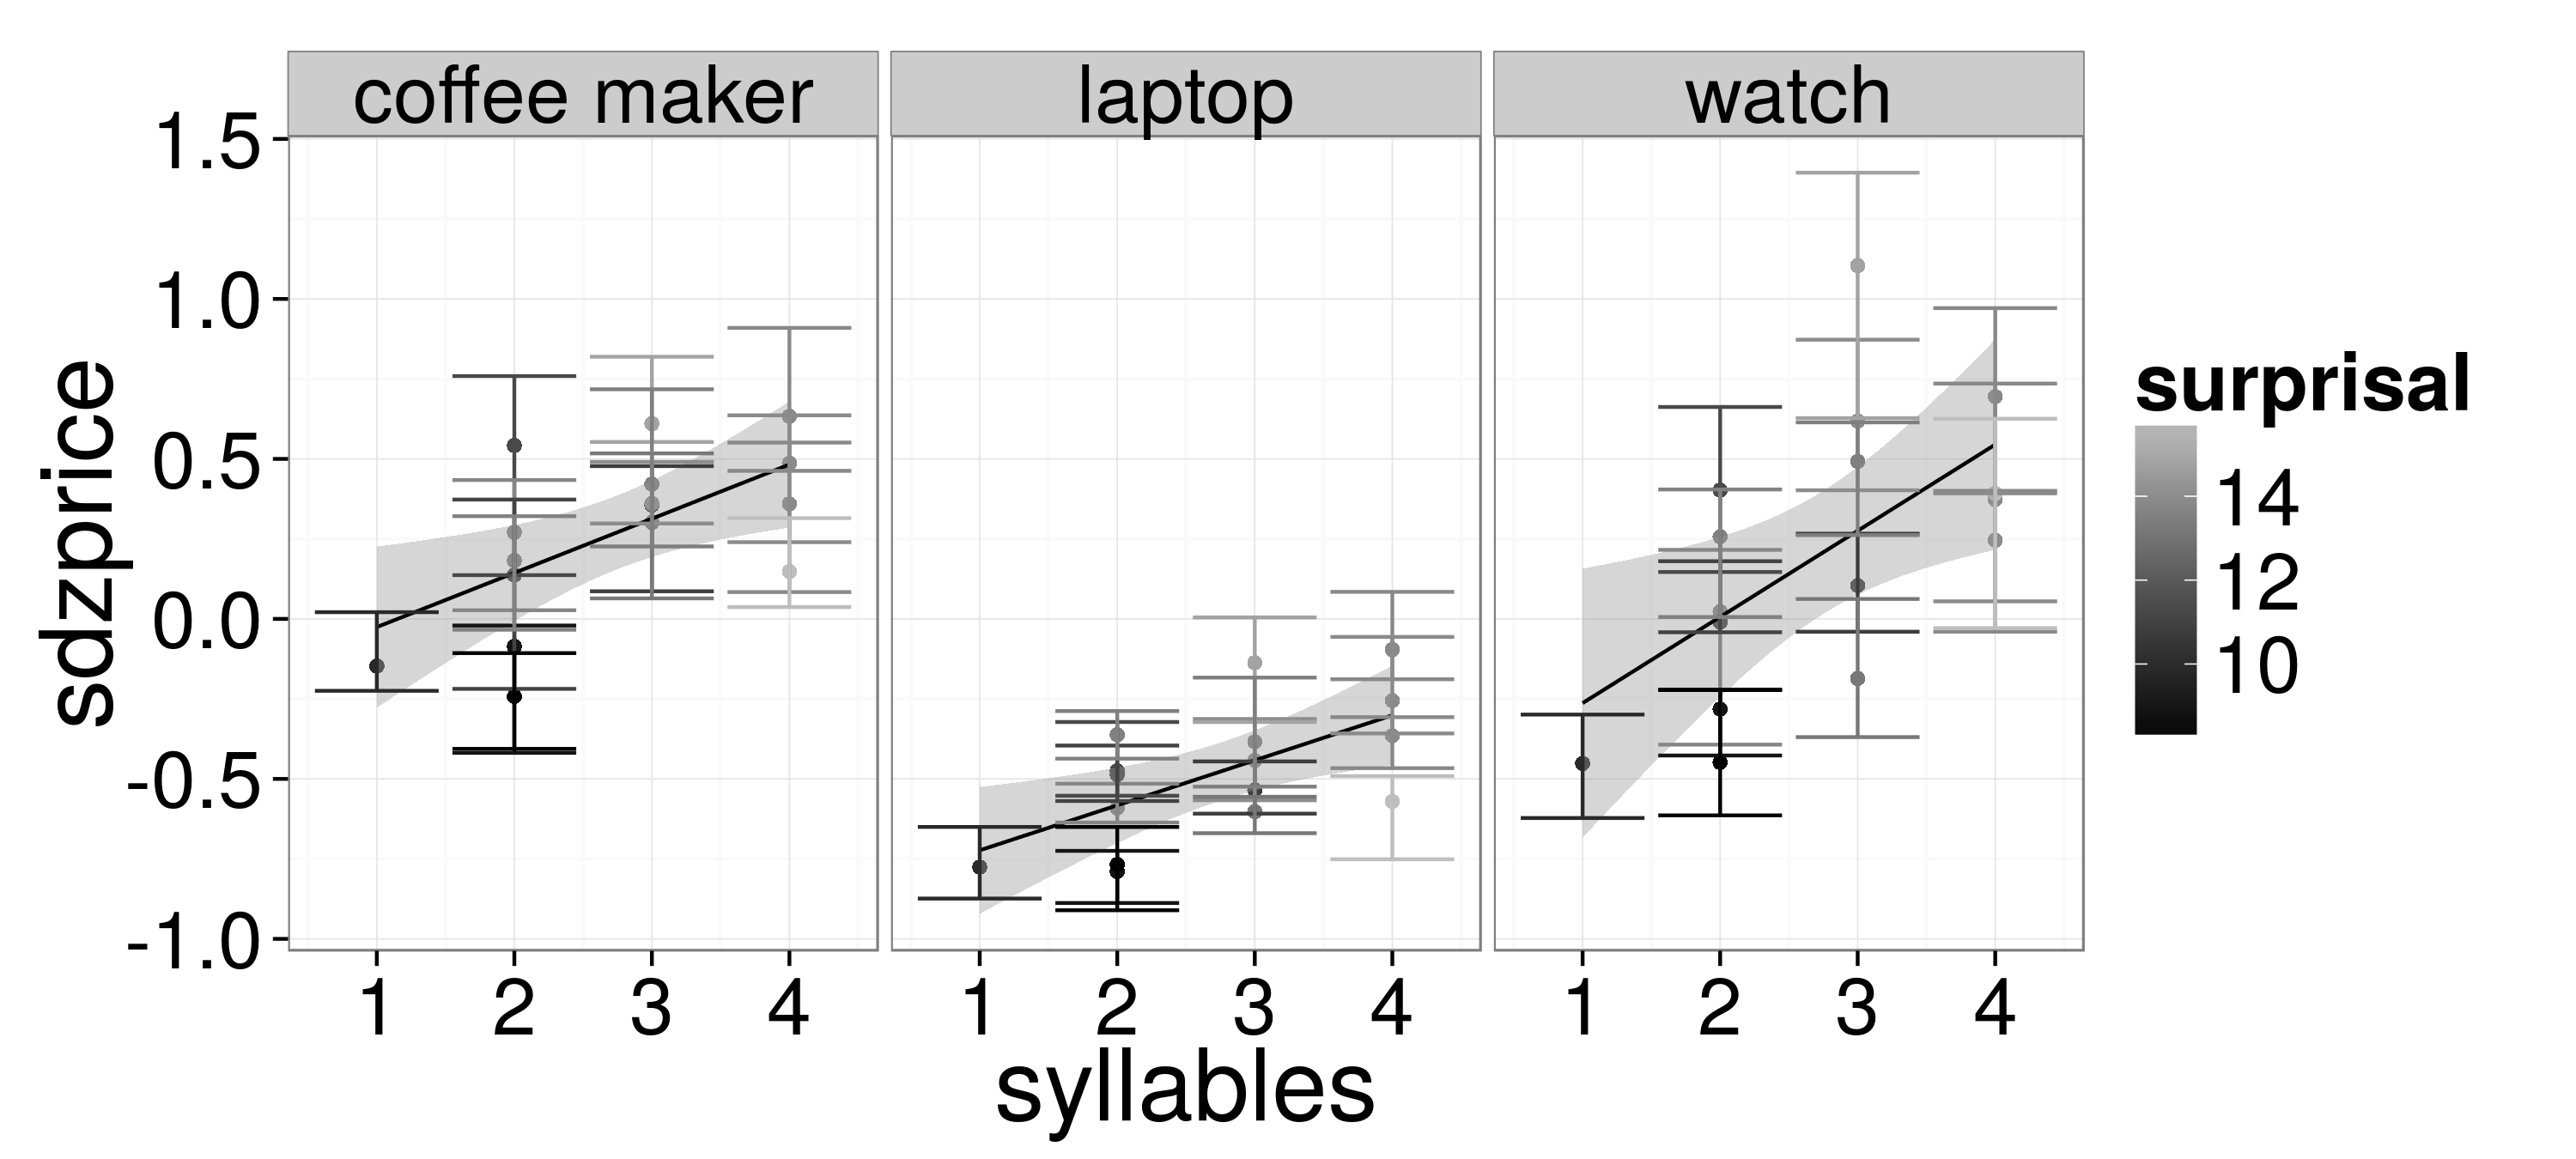
\includegraphics[width=0.45\textwidth]{exp1-scaled-syllables.png}
  \end{center}
  \caption{Syllable length versus response in rescaled, augmented data from Experiment 1. Responses increase as a function of length in syllables and of surprisal.} 
  \label{scaled-figure}
  \end{figure}
  
  We first convert participants responses to standard deviations from the mean price for each item, where these means and standard deviations are approximated from a separate set of participants. We then z-score each participant's responses. Since every participant saw every combination of intensifier and item, this z-scoring should allow us to look at participants' responses along the same scale without introducing additional confounds.
  
  \subsection{Discussion}
  
  Our results provide evidence that cost might be a factor in determining the meaning of a degree adverb. Both syllable length and surprisal predict participants' responses.
  
  One competing explanation for the role of surprisal in Experiment 1 might be that stronger degree adverbs, because they explain things that are more unusual and therefore possibly more rare and less frequently talked about, are consequently said less frequently. That is, perhaps the rarity does not cause the meaning, but rather the meaning causes the rarity. Although this explanation does not account for why syllable length should predict degree adverb strength above and beyond surprisal, we ran Experiment 2 to try to rule out this competing explanation. 
  % 
\section{Experiment 2: deintensifiers}

  If it were the case that objects that are more extreme along a scale are less common and therefore talked about less, and so the words that describe them (stronger degree intensifying adverbs) are consequently less frequent, then stronger deintensifying adverbs, which describe items more typical along a scale and therefore perhaps more common, would be more frequent in a corpus. Therefore, for deintensifying adverbs, we would again expect a positive relationship between surprisal and price (since all of our items are ``expensive'', the lower the price, the more typical an item would be along the price scale).
  
  If, on the other hand, the meaning of a degree adverb is stronger the less common it is as a result of the additional cost of uttering it, we would expect a negative relationship between surprisal and price for deintensifying adverbs.
  
  We ran Experiment 2 to disentangle these two hypotheses.

  \subsection{Method}
    \subsubsection{Participants}
    We recruited 40 participants on Amazon's Mechanical Turk.
    \subsubsection{Procedure and Materials}
      
      Our procedure was the same as in Experiment 1, except that we drew our degree adverbs from a set of 7 deintensifiers (Table~\ref{deintensifiers-table}) and added the additional item \emph{headphones}.
      
      In addition, since we had degree adverbs of varying word lengths, we used $-log(frequency)$ for each word rather than surprisal. Since these values are proportional to one another, this is sufficient for determining whether a relationship exists between surprisal and responses.
      
      The surprisals and syllable lengths of these degree adverbs were again correlated (0.4903468).
      
      \begin{table}[!ht]
      \begin{center} 
      \caption{Deintensifying degree adverbs from Experiment 2.} 
      \label{deintensifiers-table} 
      \vskip 0.12in
      \begin{tabular}{lrr} 
      \hline
      Deintensifier    &  Frequency & Syllable length \\
      \hline
      kind of & 43691232 & 2 \\ 
      a bit & 33634149 & 2 \\ 
      slightly & 28523541 & 2 \\ 
      sort of & 19227411 & 2 \\ 
      somewhat & 14075405 & 2 \\ 
      moderately & 1922506 & 4 \\ 
      a tad & 775965 & 2 \\  
      \hline
      \end{tabular} 
      \end{center} 
      \end{table}
  \subsubsection{Results}    
  
    Using the same rescaling analysis as in Experiment 1, we found no significant effect of suprisal or syllable length (Figure ~\ref{scaled-figure-exp2}, surprisal: estimate=0.0251, p=0.29; syllables: estimate=0.0162, p=0.74).
  
    \begin{figure}[ht]
    \begin{center}
    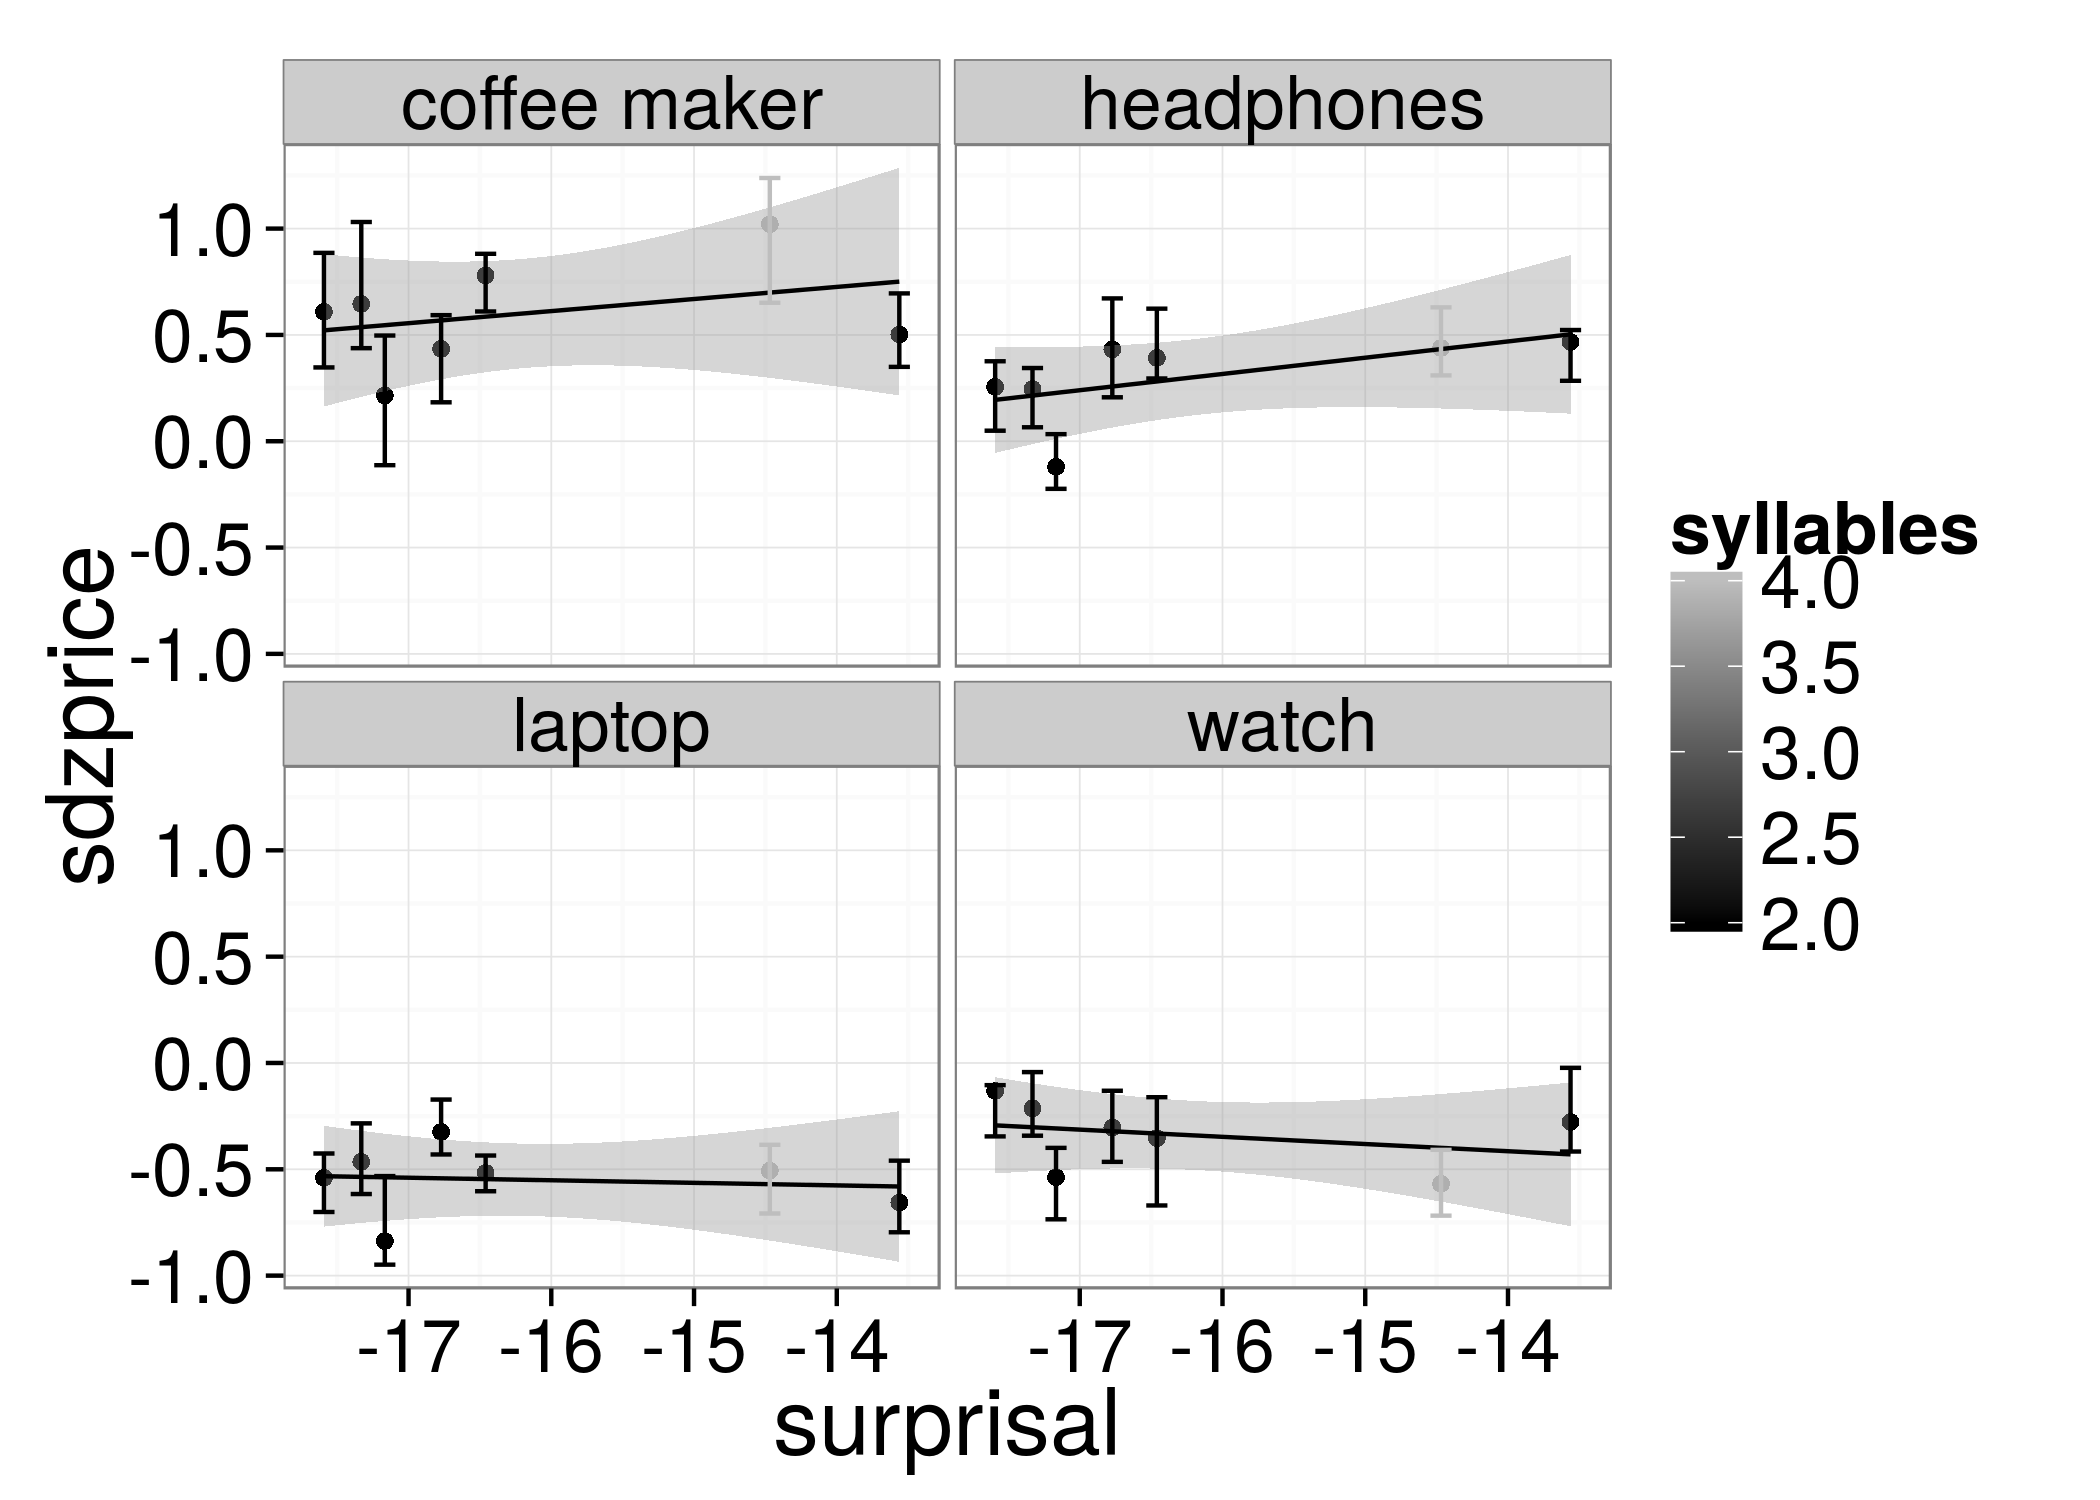
\includegraphics[width=0.45\textwidth]{exp2-scaled.png}
    \end{center}
    \caption{Surprisal versus response in rescaled, augmented data from Experiment 2.} 
    \label{scaled-figure-exp2}
    \end{figure}
  \subsection{Discussion}
  
    Our findings were inconclusive between the two hypotheses, which might indicate that neither is true, that both are true and their effects compete against each other for deintensifiers, or our assumptions about the meanings of deintensifiers are not quite right.

\section{Experiment 3: replication}
  \subsection{Method}
    \subsubsection{Participants}
      We recruited 10 participants on Amazon's Mechanical Turk.
    \subsubsection{Procedure and Materials}
    
      Our procedure was the same as in Experiment 1, but with a slightly different set of degree adverbs that included both intensifers and deintensifiers (Table~\ref{intensifiers-exp3-table}). We elicited participants' responses on only our original 3 items. We again used $-log(frequency)$ for each word rather than surprisal. The surprisals and syllable lengths of these degree adverbs were again correlated (0.5974078).
  
  \subsubsection{Results}
    In the same rescaling analysis, for intensifiers we found only a marginally significant effect of surprisal in our 10 participants (Figure ~\ref{exp3-intensifiers}, surprisal: estimate=0.07193, p=0.097; syllables: estimate=0.15853,p=0.498), and for deintensifiers we again found no effects (Figure ~\ref{exp3-deintensifiers}).
  
    \begin{figure}[ht]
    \begin{center}
    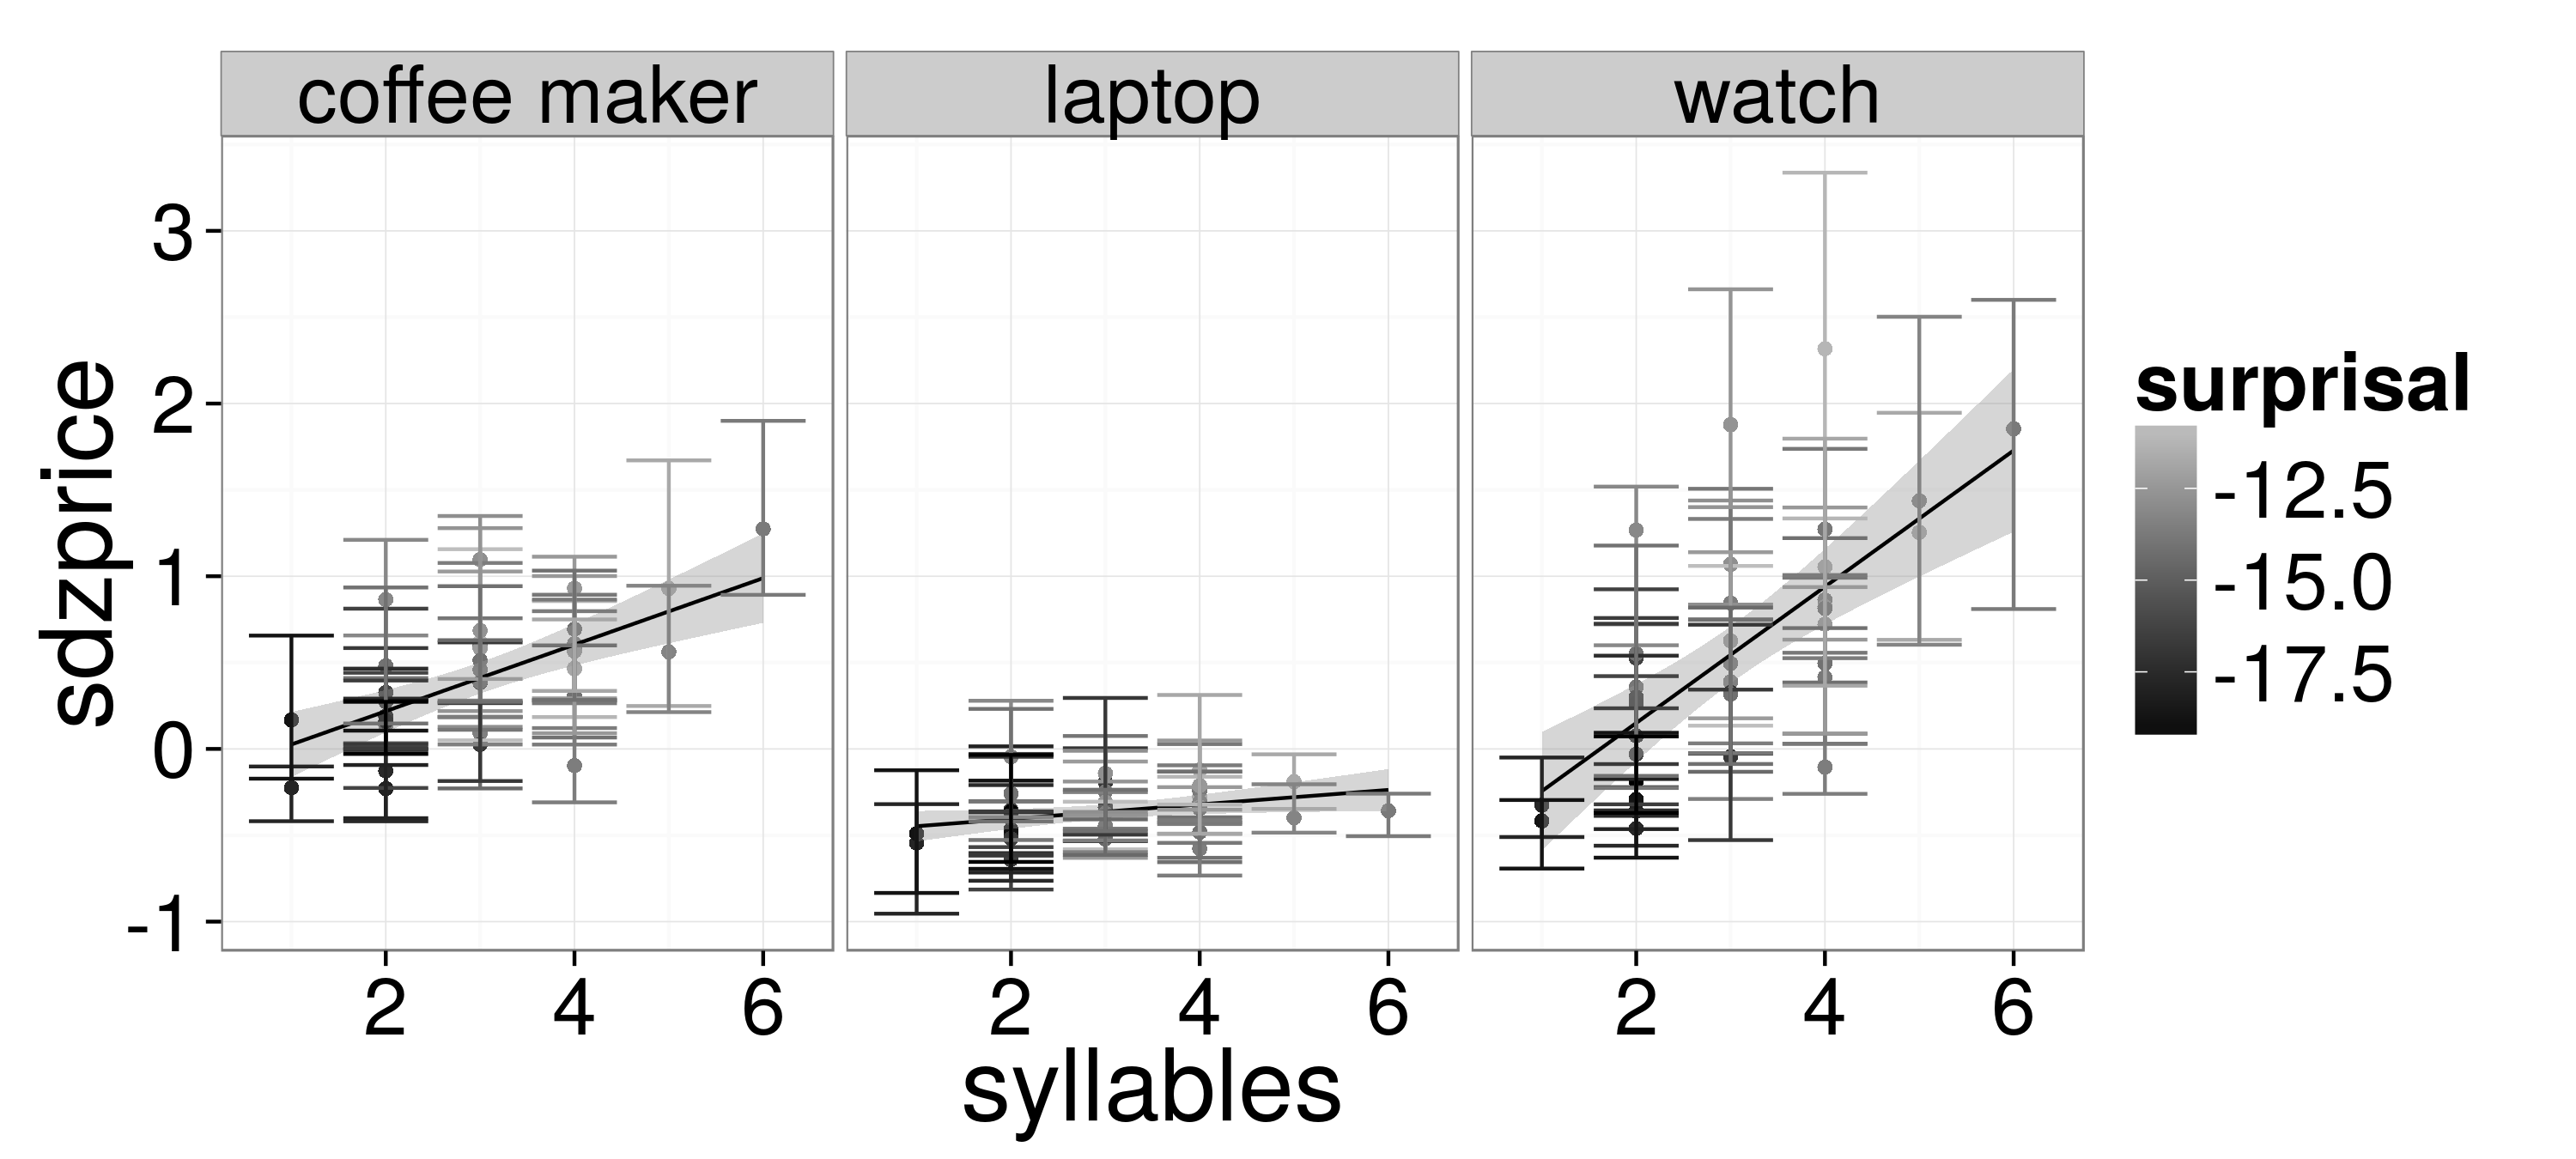
\includegraphics[width=0.45\textwidth]{exp3-intensifiers-scaled-syllables.png}
    \end{center}
    \caption{Syllable length versus response in rescaled, augmented data from Experiment 3 (slightly modified replication of Experiment 1).} 
    \label{exp3-intensifiers}
    \end{figure}
    
    \begin{figure}[ht]
    \begin{center}
    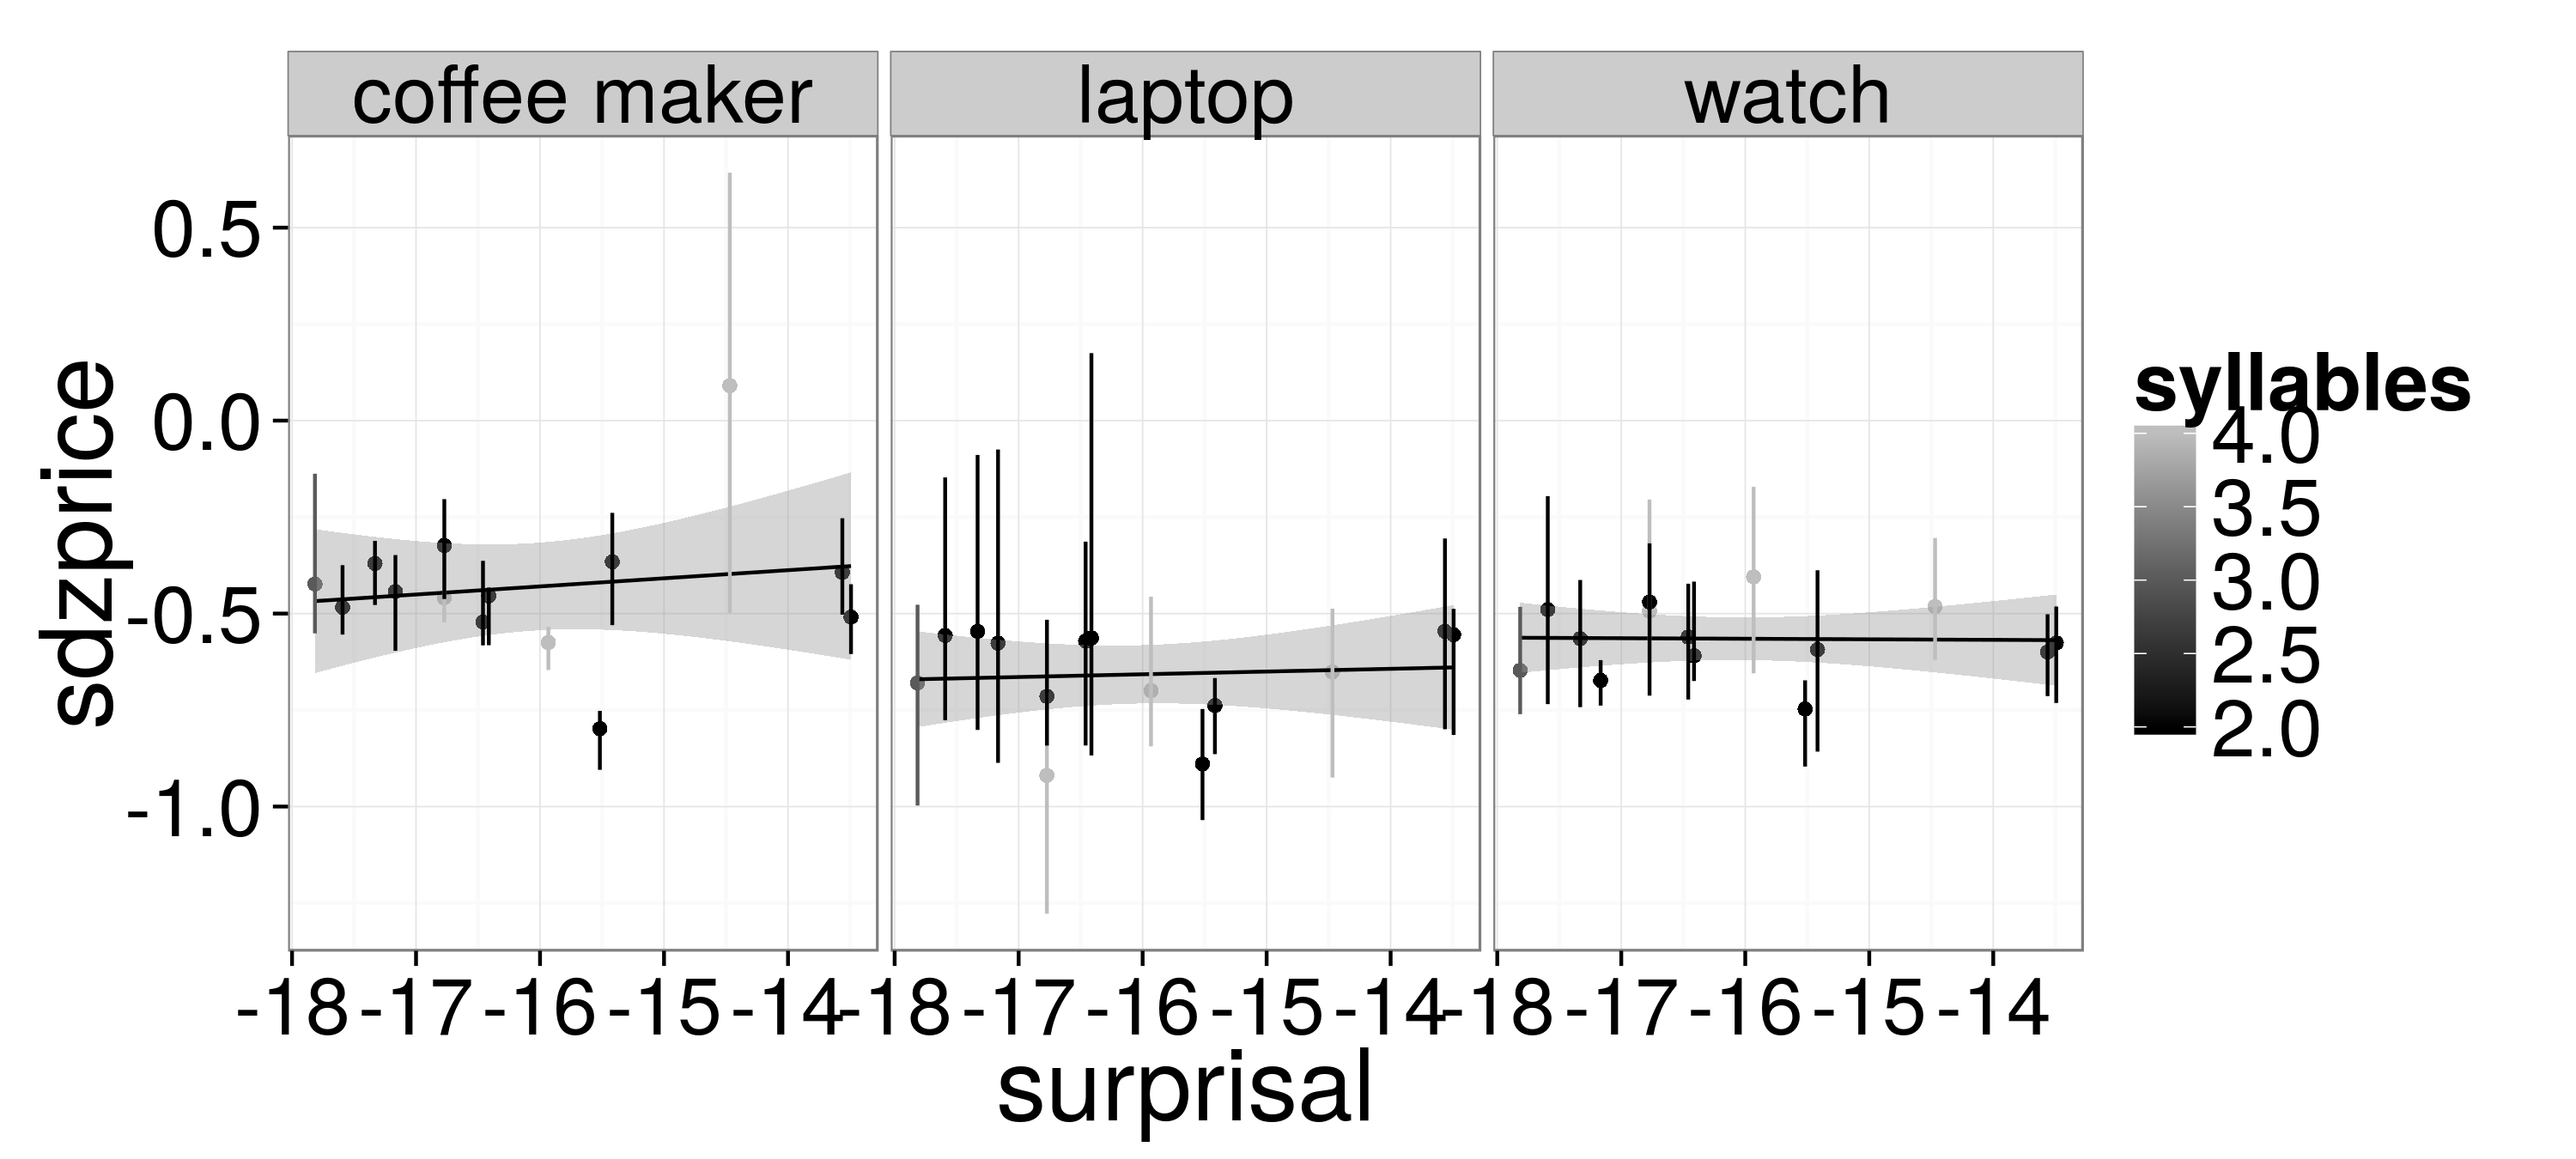
\includegraphics[width=0.45\textwidth]{exp3-deintensifiers-scaled.png}
    \end{center}
    \caption{Surprisal versus response in rescaled, augmented data from Experiment 3 (slightly modified replication of Experiment 2)} 
    \label{exp3-deintensifiers}
    \end{figure}
  
  \subsection{Discussion}
  
  We should probably run more participants on this experiment. Possibly we can elicit individuals' means and variances for each of the items, as well.
  
  \section{Conclusion}
  
  We provide some evidence that the strength of a degree adverb might be a function of the cost of that adverb.

% 
% I excluded one participant, whose answers were on average __ degrees of magnatude above all other responses.
% 
% 
% 
%   In an attempt to deconfound the findings of Experiment 1, we ran Experiment 2 on a new set of degree adverbs: deintensifying degree adverbs. We assumed that words like \emph{moderately} modify the meaning of the adjective they modify so that the object in question is closer to the average version of that object, i.e. that a ``moderately expensive laptop'' would mean ``closer to the average price of laptops than an expensive laptop''. Then the stronger this deintenfying degree adverb's meaning, the more average the object being described would be. Given this assumption, we could better test our hypothesis that degree adverbs' strength is derived from their frequency. While a strong intensifying degree adverb would describe unusual and therefore possibly infrequent items, a strong deintensifying adverb would describe more usual and therefore more frequent items.
%   
%   If infrequent degree adverbs have stronger meanings, we would expect a positive correlation between frequency and degree in the case of degree adverbs. If more frequent items are more likely to be talked about and therefore degree adverbs that describe these more frequent items are more likely to be used, then we would expect a negative correlation between frequency and degree.
%   
%   %We assumed that if the meaning of a deintensifying degree adverb was stronger, it would describe a more adverage, canonical object.
%   
%   \subsection{Method}
%     \subsubsection{Participants}
%     We recruited 10 participants on Amazon's Mechanical Turk.
%     \subsubsection{Procedure and Materials}
%   \subsection{Results}
%   \subsection{Discussion}
%   
%   Our findings in Experiment 2 might provide evidence that our findings in Experiment 1 are due to the frequencies of the items being described rather than to degree adverbs derving their meanings from their frequencies.
%   
%   However, this is inconsistent with the finding that syllable length, on top of inverse frequency, is a marginally significant predictor of intensifying degree adverb strength. It may be the case that our assumption about the meanings of deintensifying degree adverbs was flawed. Possibly deintensifying degree adverbs do not merely indicate the item in question is closer to average. We therefore ran Experiment 3 where rather than using deintensifying adverbs, we used intensifying adverbs paired with ``average'', which more likely carries the meaning we assumed deintensifiers had.
%   
% \section{Experiment 3}
% 
%   In Experiment 3, we attempted to replicate our findings about frequency and degree on a slightly refined set of degree adverbs and nouns. At the same time, we ask the same question as Experiment 2 (Are our findings in Experiment 1 due to the fact that infrequent degree adverbs consequently have stronger meanings, or due to the fact that infrequent items are less likely to be talked about?) with less uncertainty about the meanings of the sentences we give participants. 
%   
%   \subsection{Method}
%     \subsubsection{Participants}
%     \subsubsection{Procedure and Materials}
%     
%      We chose our new set of adverbs to have minimal lexical ambiguity, so that the 1-gram frequencies accurately reflect the frequency which which these words are used as modifiers of degree. We avoided adverbs that are frequently used to communicate properties independent of degree: For example, we avoided \emph{crazy} because it often communicates erratic behavior or madness and \emph{super} because is often used in the context of comic books heros.
%      
%      We also modified our set of nouns to include \emph{sweater} and \emph{headphones} (purchases we though Mechanical Turk workers would be somewhat familiar with) and to no longer included \emph{watch}. Because of the new popularity of smartwatches, \emph{watch} is now somewhat lexically ambiguous.
%      
%      Items in the replication condition were presented in the same way as in Experiment 1, and items in the new condition were changed to say ``It was a(n) [adverb] average price.''
%      
%   \subsection{Results}
%   \subsection{Discussion}
% 
% \section{Acknowledgments}
% 
% Acknowledgments.
% 
\nocite{web1t5gram}
\nocite{lewis}

\bibliographystyle{apacite}

\setlength{\bibleftmargin}{.125in}
\setlength{\bibindent}{-\bibleftmargin}

\bibliography{degree-adverbs}

      \begin{table}[!ht]
      \begin{center} 
      \caption{Intensifying degree adverbs from Experiment 3.} 
      \label{intensifiers-exp3-table} 
      \vskip 0.12in
      \begin{tabular}{lrr} 
      \hline
      Inntensifier &  Frequency & Syllable length \\
      \hline 
      very        & 292897993 & 2 \\
      really      & 148918637 & 2 \\ 
      real        & 144660526 & 1 \\ 
      rather      &  66341863 & 2 \\ 
      quite       &  55269390 & 1 \\ 
      pretty      &  43623658 & 2 \\ 
      highly      &  36460329 & 2 \\ 
      slightly    &  28523541 & 2 \\ 
      extremely   &  21862963 & 3 \\ 
      totally     &  20950052 & 3 \\ 
      truly       &  19778608 & 2 \\ 
      super       &  16902202 & 2 \\ 
      crazy       &  13048828 & 2 \\ 
      greatly     &  11337773 & 2 \\ 
      terribly    &   1906059 & 3 \\ 
      wildly      &   1414395 & 3 \\ 
      radically   &   1414254 & 4 \\ 
      amazingly   &   1384225 & 4 \\ 
      vastly      &   1311113 & 2 \\ 
      intensely   &   1084765 & 3 \\ 
      hugely      &   1074430 & 2 \\ 
      enormously  &   1011751 & 4 \\ 
      exceedingly &    977435 & 4 \\ 
      extraordinarily & 900456 & 6 \\ 
      excessively & 877280 & 4 \\ 
      horribly & 819111 & 3 \\ 
      decidedly & 817806 & 4 \\ 
      ever so & 697737 & 3 \\ 
      ridiculously & 581660 & 5 \\ 
      uber & 503592 & 2 \\ 
      insanely & 359644 & 3 \\ 
      supremely & 296134 & 3 \\ 
      fantastically & 250989 & 4 \\ 
      outrageously & 240010 & 4 \\ 
      stupidly & 224107 & 3 \\ 
      uncommonly & 135747 & 4 \\ 
      phenomenally & 120769 & 5 \\ 
      astoundingly & 73041 & 4 \\ 
      crazily & 52356 & 3 \\
      \hline
      \end{tabular} 
      \end{center} 
      \end{table}
      
      \begin{table}[!ht]
      \begin{center} 
      \caption{Dentensifying degree adverbs from Experiment 3.} 
      \label{deintensifiers-exp3-table} 
      \vskip 0.12in
      \begin{tabular}{lrr} 
      \hline
      Inntensifier &  Frequency & Syllable length \\
      \hline
      a little & 54587448 & 3 \\ 
      kind of & 43691232 & 2 \\ 
      a bit & 33634149 & 2 \\ 
      relatively & 19236549 & 4 \\ 
      sort of & 19227411 & 2 \\ 
      somewhat & 14075405 & 2 \\ 
      fairly & 13432053 & 2 \\ 
      reasonably & 8307027 & 4 \\ 
      barely & 5483661 & 2 \\ 
      kinda & 4961342 & 2 \\ 
      moderately & 1922506 & 4 \\ 
      a tad & 775965 & 2 \\ 
      sorta & 723566 & 2 \\ 
      \hline
      \end{tabular} 
      \end{center} 
      \end{table}

      %mildly is a good deintensifying adverb

\end{document}
